% CV802 Sub-project 2 -- one-page report (CVPR camera-ready style, no references).
% Build: bash surface/docs/deliverables/build_all.sh   (regenerates table.tex from results.json, then pdflatex)
\documentclass[10pt,twocolumn,letterpaper]{article}
\usepackage{cvpr}
\usepackage{microtype}
\definecolor{cvprblue}{rgb}{0.21,0.49,0.74}
\usepackage[breaklinks,colorlinks,allcolors=cvprblue]{hyperref}
\def\paperID{}\def\confName{CV802}\def\confYear{2025}
\newcommand{\pend}{\textcolor{BrickRed}{\textit{pend.}}}
\setlength{\abovedisplayskip}{2pt}\setlength{\belowdisplayskip}{2pt}
\renewcommand{\paragraph}[1]{\vspace{1pt}\noindent\textbf{#1}\hspace{0.4em}}
\makeatletter
\renewcommand\section{\@startsection{section}{1}{\z@}{-5pt plus -1pt}{2pt}{\large\bf}}
\patchcmd{\@maketitle}{\vskip .375in}{\vskip -0.05in}{}{}
\patchcmd{\@maketitle}{\vspace*{24pt}}{\vspace*{8pt}}{}{}
\makeatother
\captionsetup{skip=3pt}

\title{From Coloured Points to Printable Textured Meshes}
\author{Anas Khan \quad MBZUAI \quad {\tt\small anas.khan@mbzuai.ac.ae} \quad CV802 Sub-project 2: Surface Extraction}

\begin{document}
\pagestyle{empty}\thispagestyle{empty}
\twocolumn[{\renewcommand\twocolumn[1][]{#1}%
\maketitle\vspace{-34pt}
\begin{center}
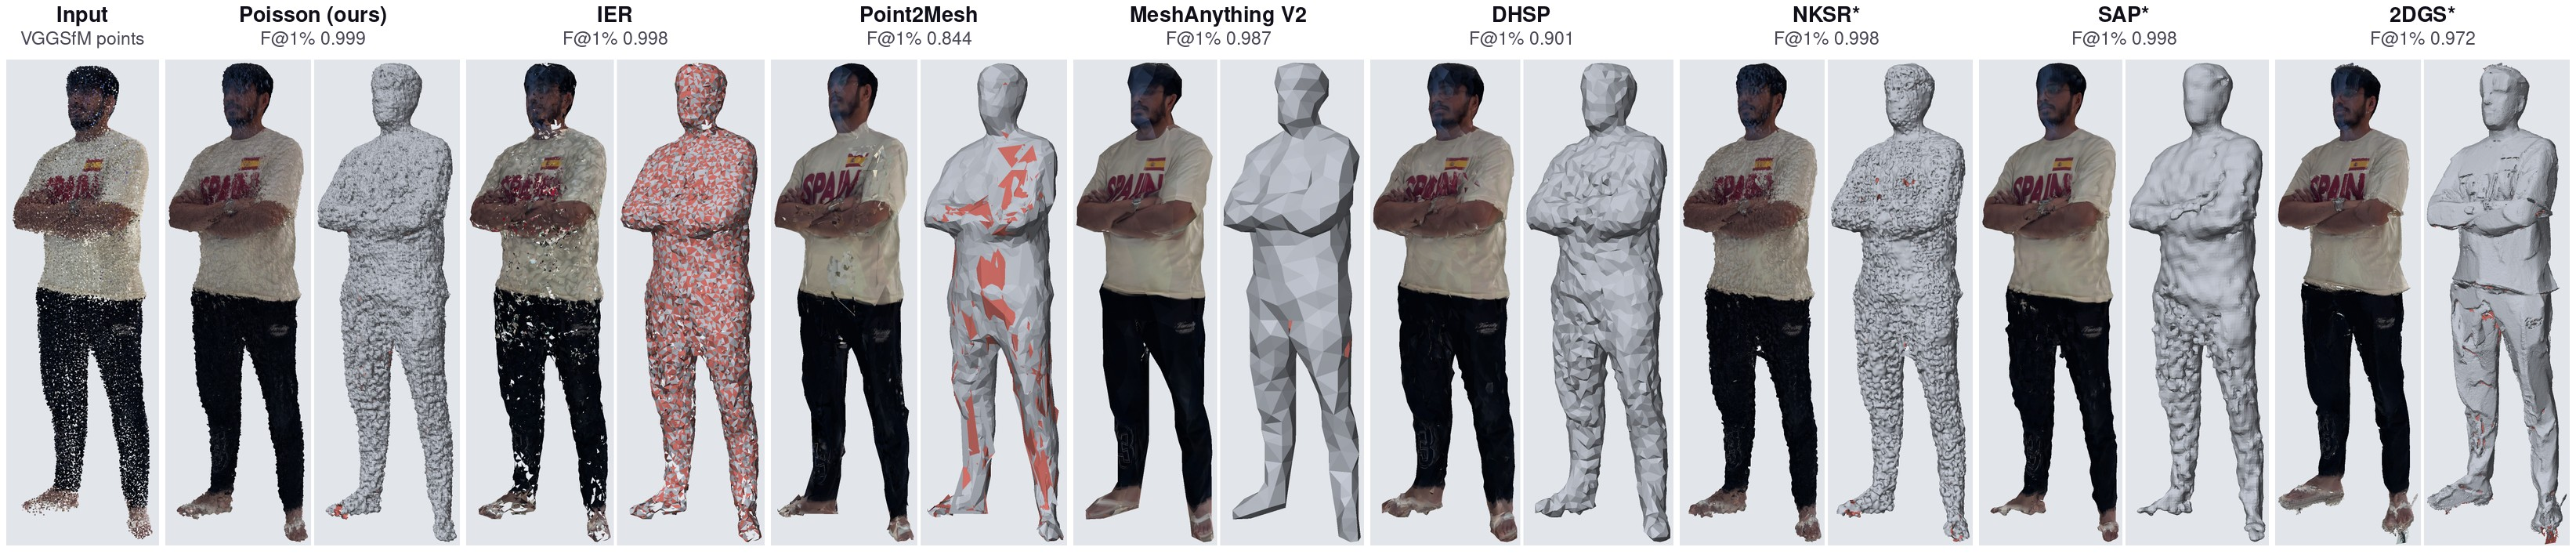
\includegraphics[width=0.93\textwidth]{../figs/fig_strip_vggsfm.jpg}\\[-2pt]
\captionof{figure}{Best mesh per method on VGGSfM: \emph{textured} (our photo projection) | \emph{shaded}. Red
faces are back-facing (inconsistent orientation).}
\label{fig:teaser}\vspace{2pt}

{\footnotesize\setlength{\tabcolsep}{4.6pt}
\begin{tabular}{@{}lr cccc cc cc c@{}}
\toprule
 & & \multicolumn{4}{c}{VGGSfM (main input, 139k pts)} & \multicolumn{2}{c}{MVS (487k pts)} & \multicolumn{2}{c}{MVS-clean} & \\
\cmidrule(lr){3-6}\cmidrule(lr){7-8}\cmidrule(lr){9-10}
Method & Faces & CD\,\%$\downarrow$ & F@1\%$\uparrow$ & F@0.5\%$\uparrow$ & NC$\uparrow$ & CD\,\%$\downarrow$ & F@1\%$\uparrow$ & CD\,\%$\downarrow$ & F@1\%$\uparrow$ & WT \\
\midrule
Poisson (ours) & 1.02M & \textbf{0.149} & \textbf{0.999} & \textbf{0.988} & 0.75 & 0.127 & 0.999 & 0.127 & 0.999 &  \\
IER & 17k & 0.187 & 0.998 & 0.975 & 0.82 & 0.120 & \textbf{1.000} & 0.123 & \textbf{1.000} &  \\
Point2Mesh & 10k & 0.553 & 0.844 & 0.530 & 0.80 & 3.977 & 0.133 & 1.298 & 0.387 & \checkmark \\
MeshAnything V2 & 1.4k & 0.295 & 0.987 & 0.858 & 0.82 & 0.518 & 0.873 & 0.438 & 0.908 &  \\
DHSP & 6.0k & 0.583 & 0.901 & 0.407 & \textbf{0.89} & 0.636 & 0.900 & 0.627 & 0.916 & \checkmark \\
\midrule
NKSR$^\ast$ & 2.09M & 0.156 & 0.998 & 0.973 & 0.75 & \textbf{0.080} & \textbf{1.000} & \textbf{0.080} & \textbf{1.000} &  \\
SAP$^\ast$ & 64k & 0.195 & 0.998 & 0.961 & 0.81 & 0.197 & 0.963 & 0.239 & 0.948 & \checkmark \\
2DGS$^\ast$ & 657k & 0.289 & 0.972 & 0.864 & 0.75 & 0.308 & 0.938 & 0.336 & 0.928 &  \\
\bottomrule
\end{tabular}\\[2pt]
\captionof{table}{Best run per method vs.\ its own input dots. CD: mean mesh--dot gap (Chamfer), \% of the scan's
diagonal, lower is better; F@$\tau$: share within $\tau$ of each other, higher is better; NC: agreement of surface
directions; WT: closed, printable. $^\ast$\,Beyond the course list.}
\label{tab:results}}

\end{center}\vspace{-4pt}}]
\thispagestyle{empty}

\section{Task and inputs}
We turn coloured points from Sub-project 1 into textured \texttt{.obj} meshes with eight methods and our own
photo texturing, browsable side by side in our three.js mesh viewer (bonus; \texttt{run\_viewer.sh}, CPU only). Inputs are the light-shirt capture as a VGGSfM cloud (139k points, cleaned with person masks; main input), a COLMAP
MVS cloud (487k points, with normals), and the MVS cloud with 404 floating outliers removed (MVS-clean). A shared finalizer adds UV atlas, texture, metrics and renders to every mesh.

\section{Method}
\paragraph{Screened Poisson (ours, no API).}
Normals: PCA on 24 neighbours, oriented along a minimum spanning tree (cost
$1-|\mathbf n_i\!\cdot\!\mathbf n_j|$), flipped outward per component. Inward normals are splatted into a field $\mathbf V$ on a $384^3$ grid, and the
indicator $\chi$ solves
\begin{equation}
\big(-\Delta + \beta S^{\top}WS\big)\chi = -\nabla\!\cdot\mathbf V + \beta S^{\top}W c,
\end{equation}
where $S$ samples $\chi$ at the points and the screening term pins it to the iso-value $c$. We use
Jacobi-preconditioned CG, coarse to fine ($96^3\!\rightarrow\!384^3$), our own marching tetrahedra (crack-free), and
trim faces more than two voxels from the data: 1.0\,M faces in 39\,s.

\paragraph{Making the course methods work on a real scan.}
\textbf{IER}: points farthest-point sampled to its training density (12.5k). \textbf{MeshAnything V2}: raw points
give F@1\%\,0.51; our Poisson mesh fed through the authors' marching-cubes input path gives 0.987.
\textbf{Point2Mesh}: the paper's \texttt{--unoriented} loss, 0.65$\rightarrow$0.84. \textbf{DHSP}: the 3D prior is
crumpled (NC 0.65) and OptCuts did not converge in 15\,h. Re-meshing first (3k/6k faces) makes OptCuts converge in
seconds, so the full pipeline (2D geometry prior, refinement, 2D texture prior) completes: NC\,0.89, own colour.

\paragraph{Extra methods and texture.} NKSR, Shape As Points and 2DGS (masked photos, TSDF mesh).
Shape-only meshes get an xatlas atlas; each texel is rasterised to a surface point and coloured from the photos with
COLMAP cameras, z-buffer visibility, person masks, weight $(\cos^4\theta\,(d/z)^2)^{8}$ and per-photo exposure gain
($4096^2$). Metrics (Tab.~\ref{tab:results}) compare each mesh with its input cloud.

\section{Findings}
\textbf{(1)} Careful classical code is competitive: our Poisson ties the best learned methods on VGGSfM; NKSR wins
on dense MVS. \textbf{(2)} Point scores hide surface quality: DHSP's prior has F@1\%\,0.999 but is crumpled; IER's
winding is inconsistent. \textbf{(3)} Input domain and outliers dominate: MeshAnything needs
mesh-like input; Point2Mesh collapses on raw MVS (0.13) and recovers after floater removal (0.39).
\textbf{(4)} Photo texture is far sharper than point colours. \textbf{(5)} SAP, DHSP and Point2Mesh are
watertight and exported as 180\,mm STL.

\end{document}
